
\begin{exercise}
  State a score theorem for weighted graphs. That is, state something like
  \begin{theorem}[Weighted Graph Score Theorem]
     Let $(a_1,\dots,a_n) \in \R_0^n$ $a_1 \geq a_2 \geq \dots \geq a_n$. There is a weighted graph
      with this score if and only if $a_1 \leq a_2 + \dots + a_n$.
  \end{theorem}
  \textbf{Remark.} This 
  is actually even simpler.
\end{exercise}


\begin{exercise}
    \begin{proof}
Suppose $v_1, v_2 , \dots, v_n$ are the corresponding vertices of $a_1, a_2, \dots, a_n$.

Weighted Graph $ \Rightarrow $ $a_1 \leq a_2 + \dots + a_n$

We can split vertices into two groups: $v_1$ and $v_2, \dots, v_n$.

    For each edge $E(u,v)$:

    If $u$ is $v_1$ and $v$ is in $v_2, \dots, v_n$, then $v_1$ gains degree of the weight and $v_2, \dots, v_n$ gain degree of the weight.

    If $u$ is in $v_2, \dots, v_n$ and $v$ is $v_1$, then $v_1$ gains degree of the weight and $v_2, \dots, v_n$ gain degree of the weight.

    If $u$ is in $v_2, \dots, v_n$ and $v$ is $v_2, \dots, v_n$, then $v_1$ gains no degree and $v_2, \dots, v_n$ gain the degree of double weight.

    Therefore, the degree of $v_1$ must be less or equal than the total degree of $v_2, \dots, v_n$, namely $a_1 \leq a_2 + \dots + a_n$.


$a_1 \leq a_2 + \dots + a_n$ $ \Rightarrow $ Weighted Graph

    \textbf{Case 1}. When $a_1 = a_2 + \dots + a_n$.

    Construct Weighted Graph by connecting an edge of weight $a_i$ between $v_1$ and $v_i$, $i \geq 2$.

    $v_1$ gains $a_2 + \dots + a_n$ degrees and $v_i$ gains $a_i$ degree(s), so there is a Weighted Graph.

    \textbf{Case 2}. When $a_1 < a_2 + \dots + a_n$.
    Let $A = a_1$, $B = a_2 + \dots + a_n$. $B - A = a_2 + \dots + an - a_1$.

    Construct Weighted Graph by connecting vertices in $v_2, \dots, v_n$ until the total left degree of $v_2, \dots , v_n$ is equal to the degree of $v_1$. Then it becomes \textbf{Case 1}.

    More concretely, we can do this by following process:

    For $v_i$, $i=n, n-1, \dots, 2$.

    When $a_i < B - A$, then connect an edge of weight $a_i$ between $v_i$ and $v_{i-1}$. $a_i$ becomes 0 and $a_{i-1}$ becomes $a_{i-1} - a_i$. And $B$ becomes $B - 2 a_i$.

    Now the new sequence is $a_1, a_2, \dots, a_{i-1}^\prime = a_{i-1} - a_i, 0, \dots, 0$. The new $B$ is $B - 2 a_i$.

    When $a_i \geq B - A$, then connect an edge of weight $\frac{B-A}{2}$ between $v_i$ and $v_{i-1}$. $a_i$ becomes $a_i - \frac{B-A}{2}$ and $a_{i-1}$ becomes $a_{i-1} - \frac{B-A}{2}$. And $B$ becomes $B - (B-A)=A$.

    Now the new sequence is $a_1, a_2, \dots, a_{i-1}^\prime = a_{i-1} - \frac{B-A}{2}, a_i^\prime = a_i - \frac{B-A}{2}, 0, \dots, 0$, $A = a_1 = B = a_2 + \dots + a_{i-1}^\prime + a_i^\prime$. So it becomes \textbf{Case 1}, we can simply connect $v_1$ with $v_i$, $i=2,3,\dots,n$.

    Since the sequence are sorted, there are no repeated weighted edges. And $B-A < B$, so there exists $v_k$ such that $a_k \geq B - A$.

\begin{center}
  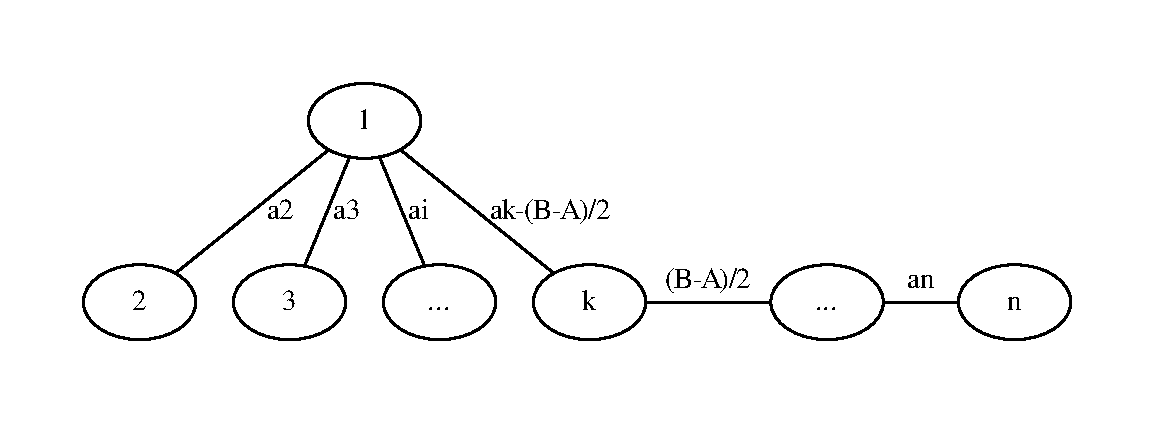
\includegraphics[width=0.5\textwidth]{figures/7-5.pdf}
\end{center}

    Therefore, we can construct a Weighted Graph if $a_1 \leq a_2 + \dots + a_n$.


    \end{proof}
\end{exercise}

